\chapter{Introduction}

\section{Motivation}

Computational Systems Biology is a growing inter-discplinary field that focuses on understanding complex biological systems. \autocite{kitano2002computational}
Traditionally, biologists would build scientific hypotheses on paper and then test them through \textit{in vitro} and \textit{in vivo} experimentation, now this work is assisted by computer software.
Systems biology is the progression of classical molecular biology from a qualitative to a quantitative science.
Software can help not only data collection and analysis, but formulate and test hypotheses through virtual experimentation.
Computational models described here are formal descriptions of a biomedical process, and in particular intracellular kinetic models described by ordinary differential equations.
A simulation is a dynamic realization of the model that describes the evolution of the process from a particular set of starting conditions, which may be tested experimentally.
Simulation experiments allow research in areas that were once difficult to approach by providing information that is difficult or impossible to measure. \autocite{edwards2001silico}
Thus, progress in Systems Biology can result in accelerated drug discovery, safer medicines, and improved understanding of pathogenesis. \autocite{kitano2010grand, mack2004can}

In other research-oriented industries where software and simulation has been integrated, such as automobile, aerospace, and telecommunication, have seen immense cost savings and increases in efficiency.
Virtual cars are "driven" and virtual aircrafts "flown" under simulated conditions before production and manufacture. \autocite{ghosh2010connecting}
Evidence suggests that the Systems Biology software and modeling tools still has some more room to grow in order to realize its full potential (for example, the pharmaceutical industry spends 25\% of revenues on research and development, almost twice that of any other R\&D industry). \autocite{economist2005models}

What are the challenges?
First, it may be a difficult task for some researchers to write models, as they are usually phrased in terms of differential or stochastic equations.
Once completed, models may be so far removed from the biological context that is hard to identify what the model is about or what assumptions were made.
Thus, these models are difficult to search for by a computer and are not readily accessible to the community.
Simulations have generated a large amount of data.
However, when the underlying simulation procedure and model are not available, these results are difficult to interpret.

The Systems Biology community is actively addressing these concerns through the development of standards.
The range of standards include the description of computational models \autocite{hucka:2002d, LloydCellML2004}, annotation of the model assumptions and constituents \autocite{novere2005minimum}, annotation of simulation experiments \autocite{kohn2008sed}, and annotation of simulation data \autocite{dada2010sbrml}.
However, these model standards and ontologies are abstract and meant primarily to be understood by computer scientists and software developers.
It is the role of software applications to help mitigate this kind of complexity.
A modeler should not have to be concerned with all these technical details and be allowed to focus on creating and analyzing the model.

Thus, it is the goal of this work to increase researcher productivity by bridge the gap between modeling standards and end users.

\subsection{Why the Web?}

The bulk of the work described in this writing is centered around the web browser as the primary user interface, so it is worth discussing why the web was chosen as the target platform.
Due to not having any experience with graphical software development at the start of this dissertation project, I surveyed the various software platforms available to invest in.
In order to make an application widely available to researchers, writing cross platform applications is a technical challenge, especially for research groups with limited software engineering resources. \autocite{cusumano1999netscape}
Cisco estimates that the number of devices connected to the Internet will swell from about 10 billion today to 50 billion by 2020. \autocite{clark2014internet}
With the advent of modern browsers, HTML5 based web applications are cross-platform, off-line capable, and perpetually updated. \autocite{o2007web}
Thus, there are attractive technical benefits to deploying applications to the web.

By virtue of expecting users to have a network connection, web applications may also be more social.
A recent study \autocite{dabbish2012social} suggests that social networks can increase productivity.
Dabbish et al. surveyed users of the open software repository GitHub, and found that transparency and collaboration through a web interface promotes user innovation, knowledge sharing, and community building.
People are social social creatures and exhibit a rich set of inferential behavior when given visible cues through an interface like GitHub.
The amount of attention a project appears to receive signals its quality, which in turn gathers more attention and critiques.
Users follow and learn from others that and strive to put out better quality work because their virtual reputation is at stake.

Scientific web applications may also change the way models and results are made available to the scientific community.
Models are often discovered through journal publications, which contain a text description of the model, static tables and charts of the results, and possibly a supplementary section with data and the encoded model description file in standard format (such as SBML or CellML).
With the rise of online journals, the viewing application is often the web browser.
The tools developed in this dissertation can allow the model and reproducible simulation results directly embedded or linked into an interactive figure in the article itself.
The hope is that eventually, 

\section{Specific Results}

Before describing this project and the results within the chapters, it is useful to first describe the grand vision of computational modeling in which this work lay the groundwork for.

Some inspiration for this vision came from observing the success of transformative consumer computing products, Google Docs for collaborative documents, Amazon EC2 for cloud computing, and GitHub for social coding.
Google Docs excels how easy the application is to use, no installation is required, all the user needs is a web browser.
Sharing work and soliciting input from collaborators is also trivial.
However, modelers require more sophisticated interfaces and functionality than a word processor.
With EC2, individuals or groups with limited resources can access a large number of computing nodes for a short period of time without needing to invest in a large amount of hardware.
However, raw computing nodes need configuration before using with bio-modeling software.
GitHub, as mentioned previously, has been shown to be a boon for the open source software community.

Inspiration also came from existing model repositories, such as BioModels Database, JWS and the CellML repository (discussed in Chapter~\ref{chap:background}).
This work will seek to extend and leverage these existing projects with a focus on an advanced interactive user interface, and active community.
Since Graphene and Carbon are designed modularly, these projects may directly integrate the technologies developed here as well.

\begin{figure}
  \centering
  \begin{subfigure}[b]{0.5\textwidth}
    \includegraphics[width=\textwidth, page=30, trim=0cm 0cm 14cm 7cm, clip=true]{images/Figures.pdf}
    \caption{Carbon may be made publicly available, its infrastructure can be scaled horizontally on to parallel nodes.
      Anyone in the community can view active projects and sign on to use the modeling tools and store their own models.
      Existing work may be forked, modified, and the changes incorporated back upstream.
      A project management system would exist such that teams could form to collaboratively work on modeling projects.
      It is be possible for the integrator of a project to hierarchically pull in components that others are working on.
      Publications may link directly to models existing within Carbon.}
    \label{Figure:carbon-public}
  \end{subfigure}
  \begin{subfigure}[b]{0.45\textwidth}
    \includegraphics[width=\textwidth, page=31, trim=0cm 0cm 17cm 9cm, clip=true]{images/Figures.pdf}
    \caption{In a private team environment, for instance at a pharmaceutical company, the same modeling can be installed on to a local cluster, providing simulation resources while remaining able to safeguard proprietary commercial information}
    \label{Figure:carbon-private}
  \end{subfigure}
  \begin{subfigure}[t]{0.45\textwidth}
    \includegraphics[width=\textwidth, page=32, trim=0cm 0cm 17cm 12cm, clip=true]{images/Figures.pdf}
    \caption{Carbon also works as a standalone desktop installation.}
    \label{Figure:carbon-single}
  \end{subfigure}
  \caption{
  The long term goal of Carbon is to become a collaborative framework which encompasses all the computational tools a modeler needs while also providing the means to establish a social network of modelers.
  }
  \label{Figure:carbon-overview}
\end{figure}

\subsection{Summary of Chapters}

Chapter~\ref{chap:background} provides a broad and in-depth review of the standards and software tools currently used in systems biology.
Chapter~\ref{chap:graphene} is focused on the rationale, features, and developmental details of Graphene, a web framework for building interactive and graphical applications.
In order to demonstrate that Graphene is indeed useful for quickly building scientific applications and easily integrated into existing ones, Chapters~\ref{chap:tidal} and \ref{chap:redox} will present two web applications that use Graphene, TiDAL and Redox.
TiDAL is an pre-existing transcription factor regulatory network analysis tool, which Graphene was integrated with.
Redox is a newly developed pathway exploration tool, built using Graphene, used to identify desirable pathways from a large pool of candidates.
Finally, in Chapter~\ref{chap:carbon}, a prototype of Carbon is demonstrated, which is a collaborative and modular framework for hosting applications and isolated workspace environments.
Here it includes a Graphene based file management and model layout app, along with an IPython Notebook interface that allows for custom scripting and model analysis.
